\documentclass[12pt,a4]{article}





\usepackage{graphicx,amsmath,amssymb,amsthm, boxedminipage,xcolor}

%\usepackage[lined,boxed]{algorithm2e}

\usepackage{algorithm}
\usepackage{algpseudocode}

%\usepackage{algorithmic}
\usepackage{algpseudocode}
\usepackage{amsmath}
\usepackage{graphics}
\usepackage{epsfig}

\newtheorem{theorem}{Theorem}[section]
\newtheorem{proposition}[theorem]{Proposition}
\newtheorem{lemma}[theorem]{Lemma}
\newtheorem{corollary}[theorem]{Corollary}
\newtheorem{definition}[theorem]{Definition}

\newtheorem*{theorem*}{Theorem}
\newtheorem*{lemma*}{Lemma}
\newtheorem*{proposition*}{Proposition}


\newtheorem{exercise}[theorem]{Exercise}
\newtheorem{exerciseD}[theorem]{*Exercise}
\newtheorem{exerciseDD}[theorem]{**Exercise}

\let\oldexercise\exercise
\renewcommand{\exercise}{\oldexercise\normalfont}

%\let\oldexerciseD\exerciseD
%\renewcommand{\exerciseD}{\oldexerciseD\normalfont}

%\let\oldexerciseDD\exerciseDD
%\renewcommand{\exerciseDD}{\oldexerciseDD\normalfont}

\newcommand{\E}{\mathbb{E}}
%\newcommand{\nth}[1]{#1^{\textsuperscript{th}}}
\newcommand{\scalar}[2]{\ensuremath{\langle #1, #2\rangle}}
\newcommand{\floor}[1]{\left\lfloor #1 \right\rfloor}
\newcommand{\ceil}[1]{\left\lceil #1 \right\rceil}
\newcommand{\norm}[1]{\|#1\|}
\newcommand{\pfrac}[2]{\left(\frac{#1}{#2}\right)}
\newcommand{\nth}[1]{#1^{\textsuperscript{th}}}
\newcommand{\core}{\textnormal{core}}



\newif\ifsolution

\solutionfalse

\newcommand{\answer}[1]{
\ifsolution
{\color{blue} #1}
\else
\fi
}



\newcommand{\poly}{\textnormal{poly}}
\newcommand{\quasipol}{\textnormal{quasipol}}
\newcommand{\ssubexp}{\textnormal{stronglySubExp}}
\newcommand{\wsubexp}{\textnormal{weaklySubExp}}
\newcommand{\simplyexp}{\textnormal{E}}
\newcommand{\expo}{\textnormal{Exp}}



\newcommand{\N}{\mathbb{N}}
\newcommand{\nn}{\mathbb{N}_0^n}
\newcommand{\R}{\mathbb{R}}
\newcommand{\Z}{\mathbb{Z}}


\definecolor{darkgreen}{rgb}{0,0.6,0}


\date{}

\title{
  Mathematical Foundations \\of \\Computer Science\\
  \vspace{3mm}
{\normalsize CS 499,	Shanghai Jiaotong University,  Dominik Scheder}
}

\begin{document}

\maketitle

%\begin{quotation}
%  You are welcome to discuss the exercises in the discussion
%  forum. Please take them serious. Doing the exercises is as important
%  than watching the videos.
%
%  I intentionally included very challenging exercises and marked them
%  with one or two ``$*$''. No star means you should be able to solve
%  the exercises without big problems once you have understood
%  the material from the video lecture. One star means it requires 
%  significant additional thinking. Two stars means it is not 
%  unlikely that you will fail to solve them, even once you have understood
%  the material and thought a lot about the exercise. Don't feel bad
%  if you fail. Failure is part of learning.
%
%  This is the first time this course is online. Thus there might be mistakes
%  (typos or more serious conceptual mistakes) in the exercises. I will be 
%  grateful if you point them out to me!
%\end{quotation}


\setcounter{section}{3}



\begin{itemize}
 \item Monday, 2018-03-19, homework handed out
 \item Sunday, 2018-03-25, 12:00: submit questions and first submissions. You'll get feedback
 until Wednesday.
 \item Sunday, 2018-03-29 (Wednesday), 18:00: submit your review of the other group's first submission.
 \item 2018-04-01: submit final solution.
\end{itemize}



\section{Pascal's Triangle Modulo 2}




Here are two early tables of the binomial coefficient:
\begin{center}
  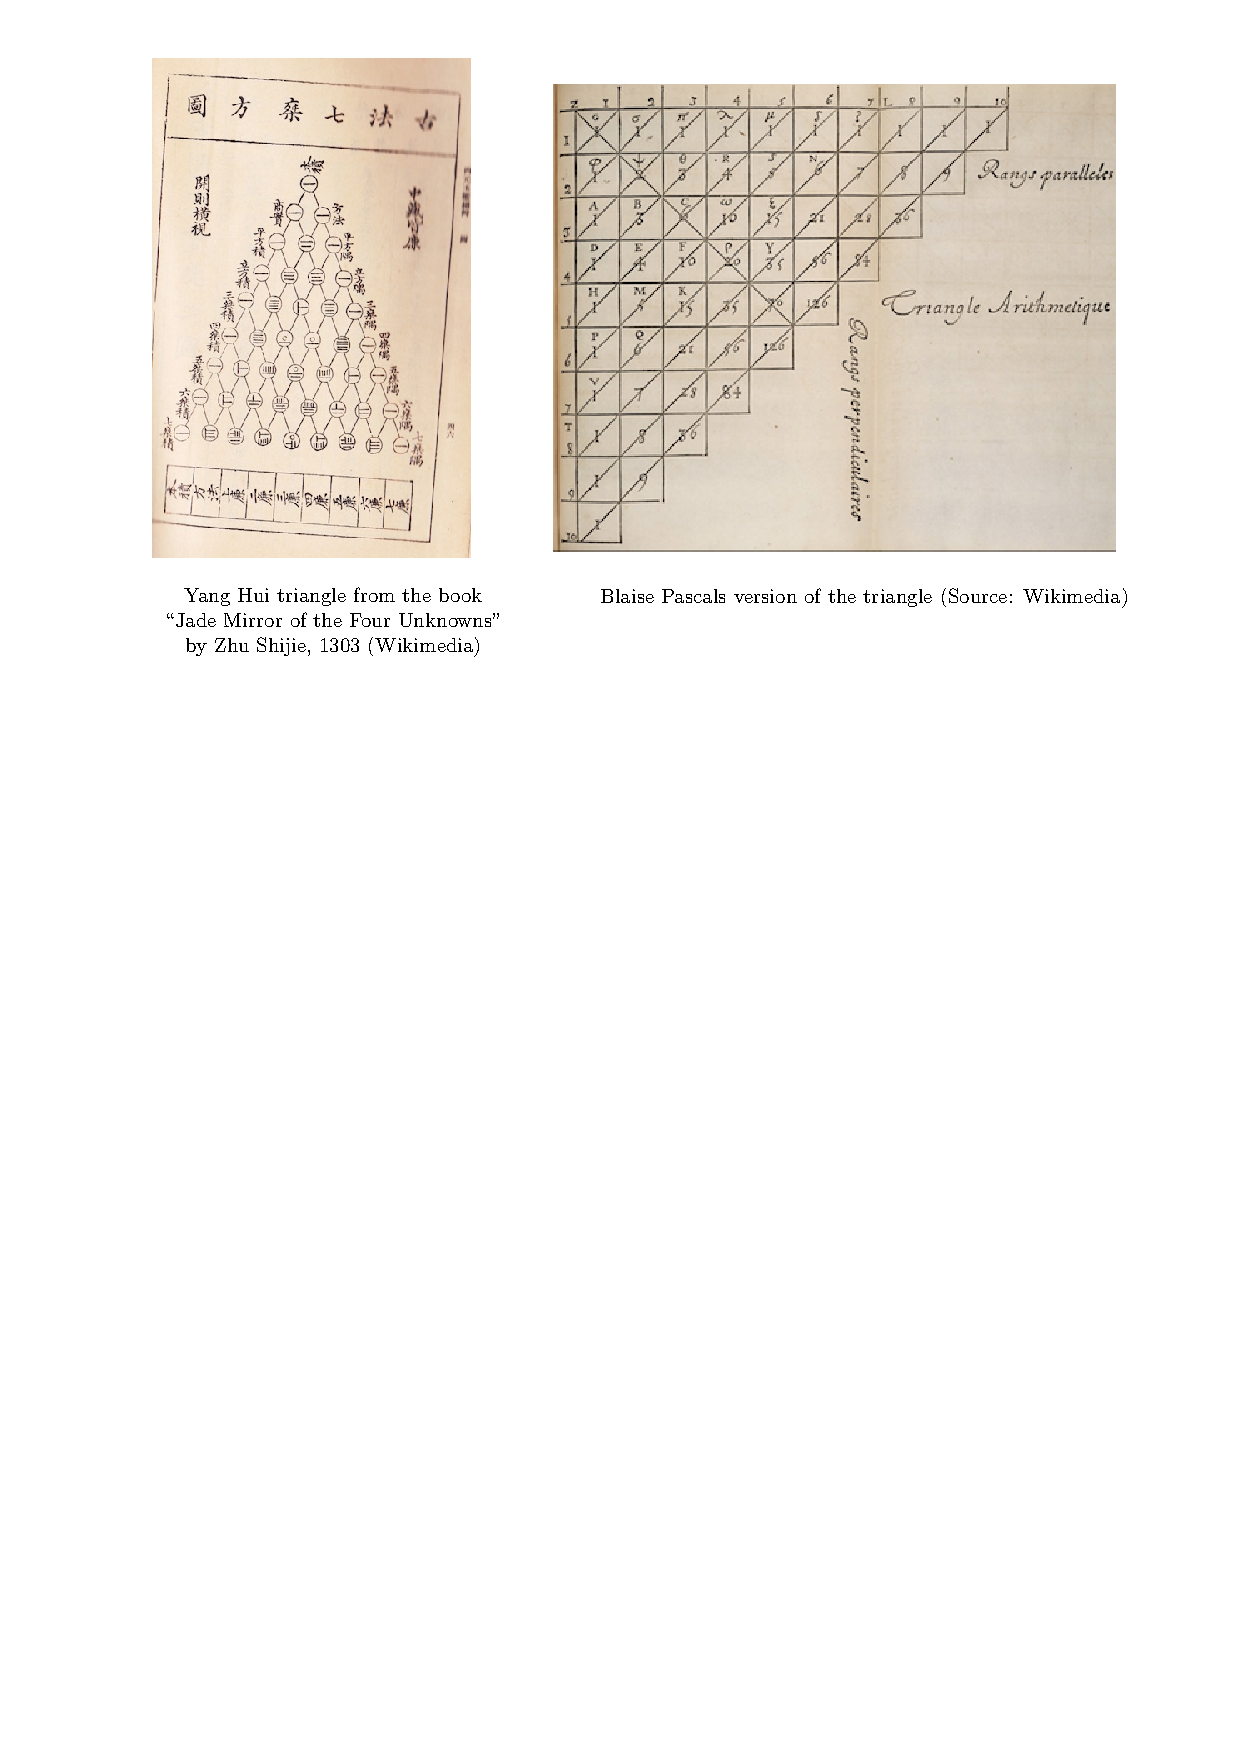
\includegraphics[width=\textwidth]{figures/two-pascal-triangles.pdf}
\end{center}
Here is my version of ``Pascal's triangle'', indicating that rows are indexes by $n$ and ``columns''
by $k$:
\begin{center}
  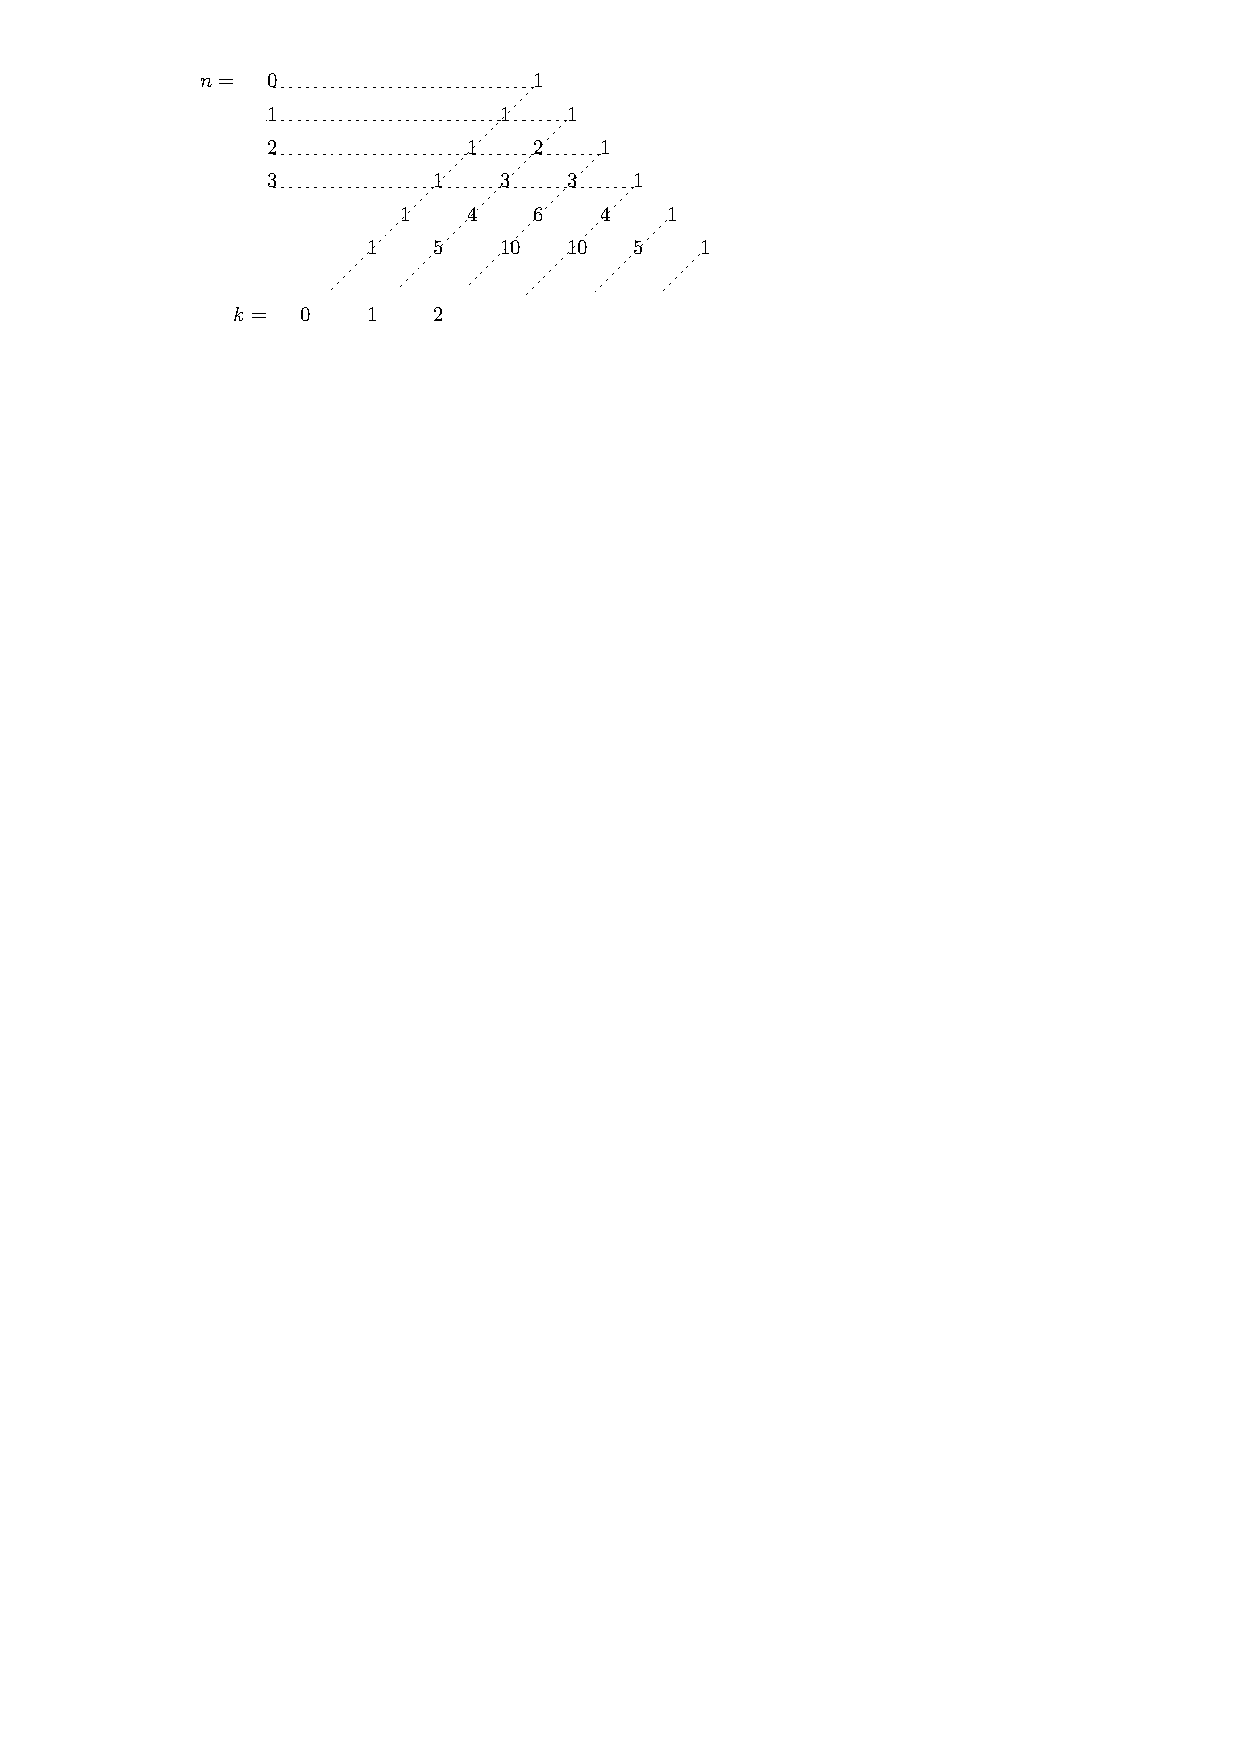
\includegraphics[width=0.8\textwidth]{figures/pascals-triangle.pdf}
\end{center}

\subsection{Lucas Theorem: ${n \choose k} \mod 2$}


Something interesting happens when we take the triangle modulo $2$, that is, we replace
even numbers by $0$ and odd numbers by $1$:
\begin{center}
  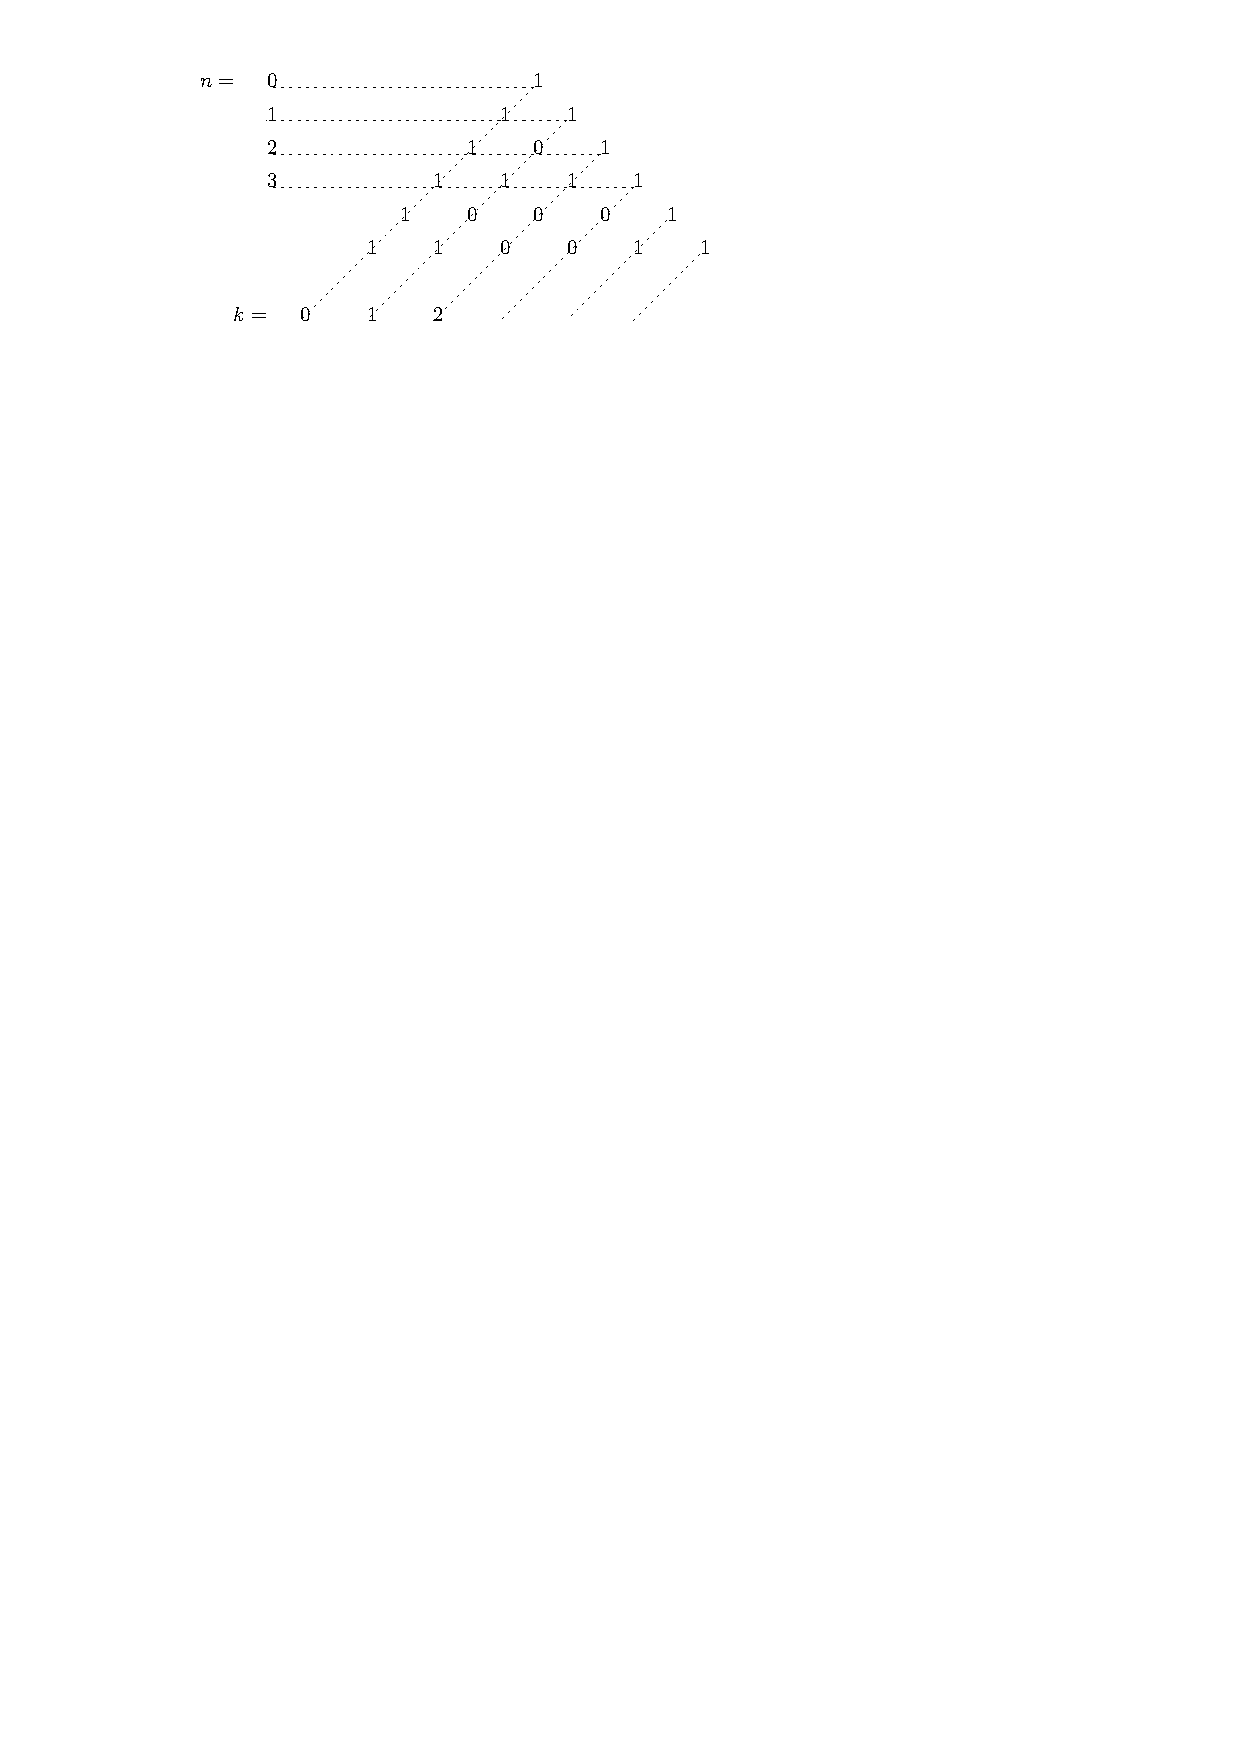
\includegraphics[width=0.8\textwidth]{figures/sierpinski-small.pdf}
\end{center}
If we draw a black dot for every $1$ and look at a larger section of this triangle, we get
the following pattern, known as the Sierpinski triangle:
\begin{center}
  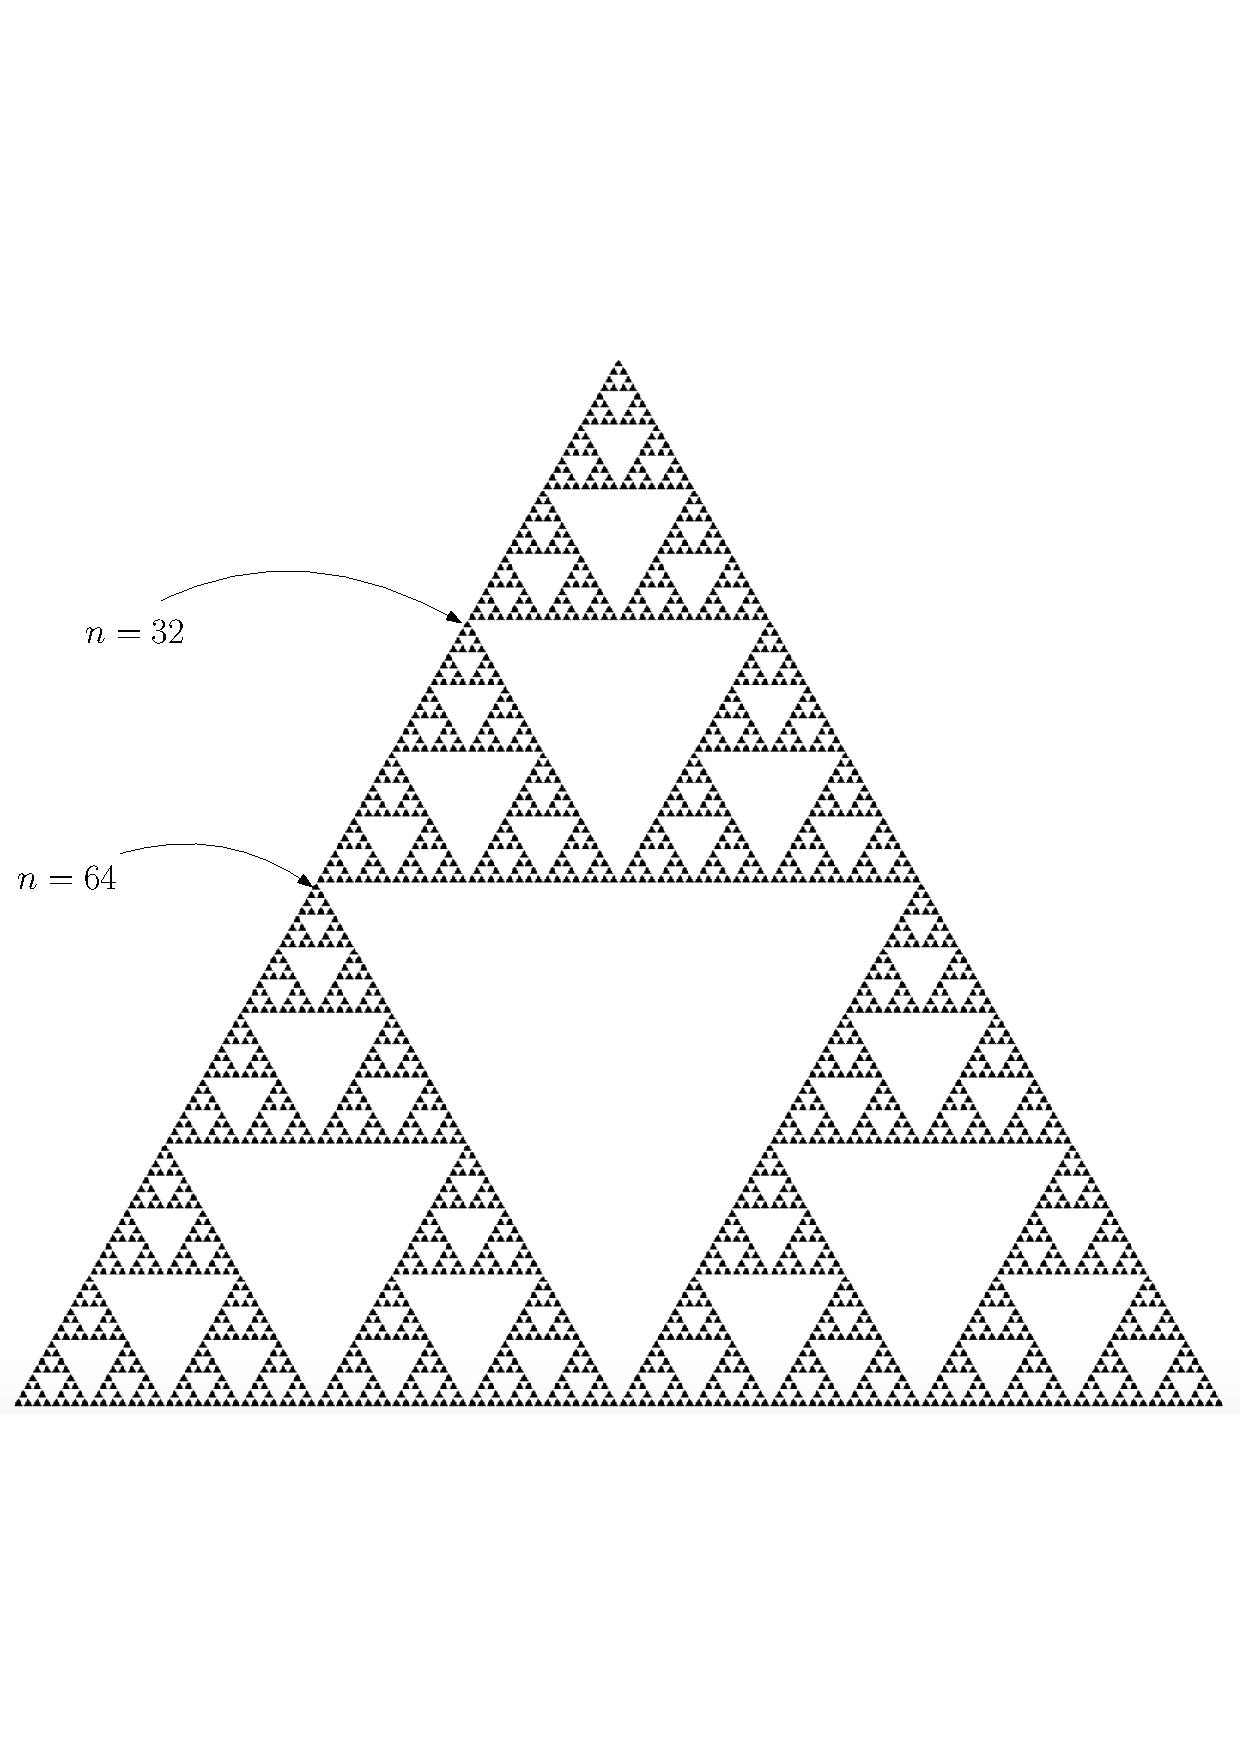
\includegraphics[width=0.8\textwidth]{figures/sierpinski-large.pdf}
\end{center}

Note the amazing recursive structure. This suggests we should be able to 
compute ${n \choose k} \mod 2$ without actually computing ${n \choose k}$,
by somehow employing this structure. In fact, here is a cool result
by \'Edouard Lucas, which we state here in a simpler, more special version:

The set $\N_0$ comes equipped with a partial ordering $\preceq$, in which
$x \preceq y$ if for every $i$, the $\nth{i}$ least significant bit of $x$ is 
at most that of $y$. Put in a simpler way, we write $x$ and $y$ as bit strings
in binary. If their length differ, we put a bunch of $0$'s in front of the smaller number
to make both strings of equal length $d$. Then we simply compare those strings
using the usual partial ordering $\preceq$ on $\{0,1\}^d$. For example,
$3 \preceq 7$ since $011 \preceq 111$, and $5 \preceq 23$ since $00101 \preceq 10111$,
but $7 \not \preceq 8$ since $0111\not \preceq 1000$.


\begin{theorem}
  Let $n, k\in \N_0$. Then ${n \choose k}$ is odd if $k \preceq n$ and even otherwise.
  \label{theorem-lucas-2}
\end{theorem}

Note that this theorem lets us compute ${n \choose k} \mod 2$ quickly for numbers $n,k$
having millions of digits, whereas no computer on Earth has the memory to evaluate 
the formula

\begin{align*}
{n \choose k} & = \frac{n \cdot (n-1) \cdot (n-2) \cdot \dots \cdot (n-k+2) \cdot (n-k+1)}
{k \cdot (k-1) \cdot (k-2) \cdot \dots \cdot 2 \cdot 1}
\end{align*}
for values that large. Let me now walk you through a proof of this theorem. 

\begin{definition}
  For a natural number $n \in \N$, let $|n|_1$ be the number of $1$'s in the binary
  representation of $n$. For example, $|1|_1 = |2|_1 = |4|_1 = 1$ but
  $|3|_1 = 2$ and $|7|_1 = 3$. 
\end{definition}

\begin{definition}
 For a natural number $a \in \N$ define $f(a)$ as the number of times the factor
 $2$ appears in $a$. Formally,
 \begin{align*}
 f(a) := \max \{ k \ | \ 2^k \textnormal{ divides } a\} \ .
\end{align*}
For example, $f(24) = 3$ since $8$ divides $24$ but $16$ does not.
\end{definition}


\begin{exercise}
   Find a closed formula for $f(n!)$ in terms of $n$ and $|n|_1$.
\end{exercise}



\begin{exercise}
   Find a closed formula for $f\left({n \choose k}\right)$ in terms of $n, k, |n|_1$, and so on.
\end{exercise}


\begin{exercise}
 Prove Theorem~\ref{theorem-lucas-2}. With our new notation, prove that
 $f\left( {n \choose k}\right)$ is $0$ if $k \preceq n$ and at least $1$ if 
 $k \not \preceq n$.
\end{exercise}



\subsection{Almost Empty Rows}

One feature of the Sierpinski triangle is that some rows are almost empty. For example, row 64
has a black dot at the very left and the very right, and only white space in between. This is because
\begin{theorem}
  Let $d \in \N_0$ and $0 < k < 2^d$. Then ${2^d \choose k}$ is even.
  \label{theorem-binomial-even}
\end{theorem}
Although this theorem follows easily from Lucas' Theorem, I want you to think about an alternative proof.
Intuitively, if some number is even, then one suspects it can be proved by ``pairing things up'' perfectly.
After all, if you can prove that in a set $S$, every element can be ``married'' to another element,
you have partitioned $S$ into couples and thus $|S|$ must be even. So let's see whether
there is a proof of Theorem~\ref{theorem-binomial-even} along these lines.
This is also
valuable because it lets you practice with notions of sets and functions. \\

Consider
the set $\{0,1\}^d$. You can view this as the set of all binary strings of length $d$.
This set has size $2^d=n$.
For $1 \leq i \leq d$ and $x \in \{0,1\}^d$ let $f_i(x)$ be $x$ with the $\nth{i}$ position
flipped. For example, $f_3(11011) = 11111$.

\begin{exercise}
 Show that $f_i$ is an involution without a fixed point.
 That is, $f(f(x)) = x$ and $f(x) \ne x$ for all $x \in \{0,1\}^d$.
\end{exercise}

\begin{proof}
According to definition, $f_i(x)$ is x with $i^{th}$ position flipped, so $f_i(x) \neq x$. And $f_i(f_i(x))$ is x with $i^{th}$
position flipped twice, which goes back to x, so $f_i(f_i(x)) = x$.Therefore, $f_i$ is an involution without a fixed point.\\
\end{proof}

Let $S \subseteq \{0,1\}^d$. We define  $f_i(S)$ as the set arising from applying
$f_i$ to every element of $S$. Formally,
\begin{align*}
f_i(S) := \{ f_i(x) \ | \ x \in S \} \ .
\end{align*}
Given a set $S \subseteq \{0,1\}^d$, we call an index $i \in [n]$ {\em active} for $S$
if $f_i(S) \ne S$. 
\begin{exercise}
Let $d=3$ and $S = \{000, 100\}$. Which of the indices $1,2,3$ are active?
\end{exercise}

\begin{proof}
Let least significant digit be the 1'st position.\\
\[f_1(S) = \{001,101\} \neq S\]
\[f_2(S) = \{010,110\} \neq S\]
\[f_3(S) = \{100,000\} = S\]
So 1 and 2 are active.
\end{proof}

\begin{exercise}
 Show that $f$ is an involution. That is, $f(f(S)) = S$. Furthermore, show that
 the only fixed points of $f$ are $\emptyset$ and $\{0,1\}^d$.
\end{exercise} 

\begin{proof}
\[\forall x \in S, f(f(x)) = x \Rightarrow f(f(S))=S\]
If $S= \emptyset$, $f(S)=S$.If there is at least one element in S and $f(S)=S$. We call the element as $x_{0\ldots 00}$. Since $f(S) = S$, $f_1(x) \in S$, which is named as $x_{0\ldots 01}$.Then, $f_2(x), f_2(x_1) \in S$, which is named as $x_{0\ldots 10} \: and\: x_{0\ldots 11}$.Similarly, we can deduce that $x_{0\ldots 00},x_{0\ldots01},x_{0\ldots 10}\ldots ,x_{1\ldots 11} \in S$, which means $S = \{0,1\}^d$. So $f(S)=S \Rightarrow S=\emptyset \: or\: \{0,1\}^d$. That is to say that the only fixed points of $f$ are $\emptyset$ and $\{0,1\}^d$.
\begin{center}
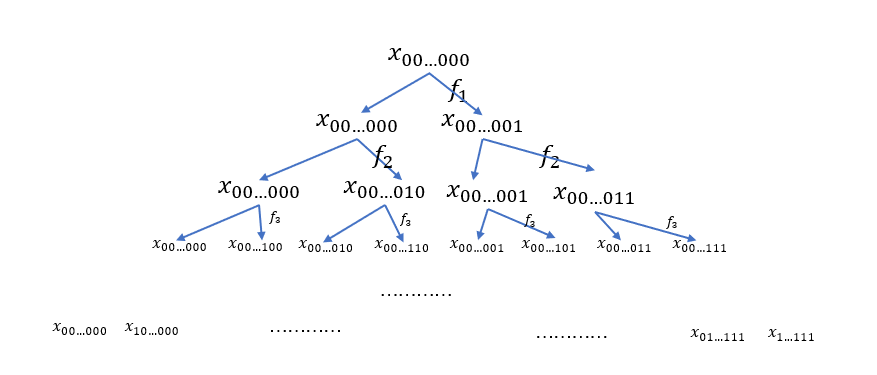
\includegraphics[scale=0.8]{10.png} 
\end{center}
\end{proof}

\begin{exercise}
   Let $\mathcal{S} = { \{0,1\}^d \choose k }$. This is a set of sets, and each set $S \in \mathcal{S}$
   consists of exactly $k$ strings from $\{0,1\}^d$. Prove the following statements: 
   \begin{enumerate}
   \item $f$ is a bijection from $\mathcal{S}$ to $\mathcal{S}$.
   \item For $1 \leq k \leq 2^d-1$, this bijection is an involution
   without fixed points.
   \item $|\mathcal{S}|$ is even for $1 \leq k \leq 2^d-1$.
   \end{enumerate}
\end{exercise}

\begin{proof}
1. $\forall S \in \mathcal{S}$, f(S) also consists of k strings, which means $f(S) \in \mathcal{S}$. So f is a bijection from $\mathcal{S}$ to $\mathcal{S}$.
\end{proof}

\begin{proof}
2. According to Exercise 4.10, For $1 \leq k \leq 2^d-1$, which means $S \neq \emptyset \: and\: S \neq \{0,1\}^d$, $f(S) \neq S$.So f is an bijection without fixed point.
\end{proof}

\begin{proof}
3. Since $f(S)\neq S$and $f(f(S))=S$, we say every S can be "married" with f(S).Thus,$|\mathcal{S}|$ is even for $1 \leq k \leq 2^d-1$.
\end{proof}




\begin{exercise}
  Complete the proof of Theorem~\ref{theorem-binomial-even}.
\end{exercise}

\begin{proof}
$$ \lvert \{0, 1\}^d \rvert = 2^d $$
$$ \lvert S \rvert = k $$ 

So every $ S $ can be considered as a choice of selecting $k$ strings from $2^d$ strings. The number of $S$ is the choices.

Thus, $${2^d \choose k} = \lvert \mathcal{S} \rvert$$ 

Since we prove that $\lvert \mathcal{S} \rvert$ is even for $1 \leq k \leq 2^d - 1$ in Exercise 4.12, ${2^d \choose k}$ is even for $0 < k < 2^d$.
\end{proof}



\begin{exerciseD}
  Generalize the above ``combinatorial'' proof to show the following theorem:
  \begin{theorem}
 Let $n = p^d$ where $p$ is a prime number. Then $p$ divides
 ${n \choose k}$ unless $k=0$ or $k=n$. 
 \end{theorem}
\end{exerciseD}

\begin{solution}

Consider the set $\{0,1, \dots, p-1\}^d$. We view this as the set of all $p$-based strings of length $d$. This set has size $p^d = n$. For $1 \leq i \leq d$ and $x \in \{0,1, \dots, p \}^d$ let $f_i(x)$ be $x$ with the $i_{th}$ position $\hat k = (k + 1) \mod p$. For example, when $p = 6 $, $f_3(12345) = 12445$, $f_3(12545)=12045$

\textbf{Step 1} 

Let's prove that $f_i$ is an involution without a fixed point. That is, $f(\dots f(x)) = f^p(x) = x$ and $f(x) \neq x$ for all $x \in \{0,1, \dots, p-1 \}^d$.

\begin{proof}
Since number at the $i^{th}$ position is changed, obviously, $f(x) \neq x$.

For the number of the $t^{th}$ position, after $p$ functions, $\hat k = ((k+1) \mod p \dots + 1) \mod p = (k + p) \mod p = k$, so $f^p(x) = x$.
\end{proof}

\textbf{Step 2} 

Let $S \subseteq \{0,1, \dots, p-1 \}^d$. Define $f_i(S) := \{ f_i(x) | x \in S\}$. We call an index $i \in [n]$ $active$ for $S$ if $f_i(S) \neq S$.

Let's prove that if $S \neq 0$ and $S \neq \{0,1, \dots, p-1 \}^d$ then $S$ has at least one active index.

\begin{proof}
Contradiction.

If $S$ has no active index, then $\forall i, f_i(S) = S$.

Since $S \neq 0$, $\exists \xi \in S$. So $f_i(\xi), f_i(f_i(\xi)), \dots, f^{d-1}_i(\xi) \in S$. Thus, every position can be number $0, 1, \dots, p-1$, which contradicts $S \neq \{0, 1, \dots, p-1\}^d$.
\end{proof}

\textbf{Step 3}

Given $S \subseteq \{0,1, \dots, p-1\}^d$, define $f(S)$ as follows: if $S = \emptyset$ or $S = \{0,1, \dots, p-1\}^d$ define $f(S) = S$. Otherwise, let $f(S) := f_i(S)$ where $i$ is the smallest active index of $S$.

Let's prove that $f$ is an involution. That is, $f(\dots f(S)) = f^d(S) = S$. Furthermore, let's prove that the only fixed points of $f$ are $\emptyset$ and $\{0,1\}^d$.

\begin{proof}
$\forall x \in S$, since $f^d(x) = x$, $f^d(x) \in S$. So $f^d(S) = S$.

Since $f(S) = S$ for $S = \emptyset$ or $S = \{0,1, \dots, p-1\}^d$, $\emptyset$ and $\{0,1, \dots, p-1\}^d$ are fixed points.

According to the last step, $f(S) \neq S$ for $S \neq \emptyset$ and $S \neq \{0,1, \dots, p-1 \}^d$, so $\emptyset$ and $\{0,1, \dots, p-1\}^d$ are the only fixed points.
\end{proof}

\textbf{Step 4}

Let $\mathcal{S} = { \{0,1, \dots, p-1\}^d \choose k }$. This is a set of sets, and each set $S \in \mathcal{S}$
consists of exactly $k$ strings from $\{0,1, \dots, p-1\}^d$. Let's prove the following statements: 
   \begin{enumerate}
   \item $f$ is a bijection from $\mathcal{S}$ to $\mathcal{S}$.
   \begin{proof}
   $\forall S \in \mathcal{S}, f(S)$ is also a set consisting of exactly $k$ strings from $\{0,1, \dots, p-1\}^d$, so $f(S) \in \mathcal{S}$. Thus, $f$ is a bijection from $\mathcal{S}$ to $\mathcal{S}$.
   \end{proof}
   \item For $1 \leq k \leq p^d-1$, this bijection is an involution without fixed points.
   \begin{proof}
   $f^d(S) = S$ as showed in \textbf{Step 3}, so $f$ is an involution.

   Since $1 \leq k \leq p^d - 1$, $\forall S \in \mathcal{S}$, $S \neq \emptyset$ and $S \neq \{0, 1, \dots, p-1\}^d$. Thus, $f(S) \neq S$. This bijection has no fixed points.

   \end{proof}
   \item $|\mathcal{S}|$ can be divided by $p$ for $1 \leq k \leq p^d - 1$.
   \begin{proof}
   $\forall S \in \mathcal{S}$, $f(S), f(f(S)), \dots f^{d-1}(S)$ construct a cluster of size $p$. $f$ can transform $S$ within the cluster and cannot transform out of the cluster, so the clusters are independent to each other. The number of clusters $\mathcal{S}$ have is an integer, so $\lvert \mathcal{S} \rvert$ can be divided by $p$.
   \end{proof}
   \end{enumerate}

   \textbf{Last Step}

\begin{proof}
When $k=0$ or $k=n$, ${n \choose k} = 1$ cannot be divided by $p$.

$$ \lvert \{0, 1, \dots, p-1\}^d \rvert = p^d = n $$
$$ \lvert S \rvert = k $$ 

So every $ S $ can be considered as a choice of selecting $k$ strings from $n$ strings. The number of $S$ is the choices.

Thus, $${n \choose k} = \lvert \mathcal{S} \rvert$$ 

Since we prove that $\lvert \mathcal{S} \rvert$ can be devided by $p$ for $1 \leq k \leq p^d - 1$ , ${n \choose k}$ can be divided by $p$ unless $k=0$ or $k=n$.
\end{proof}


\end{solution}



\end{document}
